\section*{Part A -- Graph Creation and Modification (30 pts)}

\subsection*{Q1: Graph Creation (15 pts)}

The graph shown in the assignment is an undirected graph on the ten vertices
$V=\{0,1,\dots,9\}$. Reading the edges off the figure gives $|E|=15$ edges:

\[
E=\left\{
\begin{array}{lllll}
(0,1), & (0,4), & (0,5), & (1,2), & (1,6),\\
(2,3), & (2,7), & (3,4), & (3,8), & (4,9),\\
(5,7), & (5,8), & (6,8), & (6,9), & (7,9).
\end{array}
\right\}
\]

Equivalently, as an adjacency list:

\begin{center}
\begin{tabular}{cl@{\qquad}cl}
\toprule
Node & Neighbours & Node & Neighbours \\
\midrule
$0$ & $1,\,4,\,5$ & $5$ & $0,\,7,\,8$ \\
$1$ & $0,\,2,\,6$ & $6$ & $1,\,8,\,9$ \\
$2$ & $1,\,3,\,7$ & $7$ & $2,\,5,\,9$ \\
$3$ & $2,\,4,\,8$ & $8$ & $3,\,5,\,6$ \\
$4$ & $0,\,3,\,9$ & $9$ & $4,\,6,\,7$ \\
\bottomrule
\end{tabular}
\end{center}

\paragraph{Construction.} The graph was built in NetworkX by creating an empty
undirected graph, adding the ten nodes $0,\dots,9$, and then adding the fifteen
edges listed above:

\begin{center}
\ttfamily
G = nx.Graph()\\
G.add\_nodes\_from(range(10))\\
G.add\_edges\_from(E)
\end{center}

\paragraph{Checks on the transcription.} Every vertex has degree exactly $3$, so
the graph is $3$-regular and the handshake lemma is satisfied:
$\sum_{v} \deg(v) = 30 = 2|E| = 2\cdot 15$. The graph is connected, has no
triangles, and has girth $5$. In fact these fifteen edges reproduce the
\emph{Petersen graph} (checked with NetworkX's \texttt{is\_isomorphic}
against \texttt{petersen\_graph()}, which returns
\texttt{True}), the standard $3$-regular, girth-$5$ graph on ten
vertices. Landing on the Petersen graph is a strong confirmation that the edge
list was read off the drawing correctly.

One edge deserves comment, because the drawing in the assignment is misleading
at that point: vertices $5$, $4$ and $8$ are very nearly collinear, and the
single edge $(5,8)$ is drawn passing straight across the disc of vertex $4$.
It therefore \emph{looks} like a pair of edges $(5,4)$ and $(4,8)$, but it is
one edge; if it were two, vertices $5$, $4$ and $8$ would all have degree $4$
and the graph would not be $3$-regular. In
Figure~\ref{p1:fig:q1} the edge $(5,8)$ is drawn with a slight bow so that it
visibly passes clear of vertex $4$.

\begin{figure}[H]
  \centering
  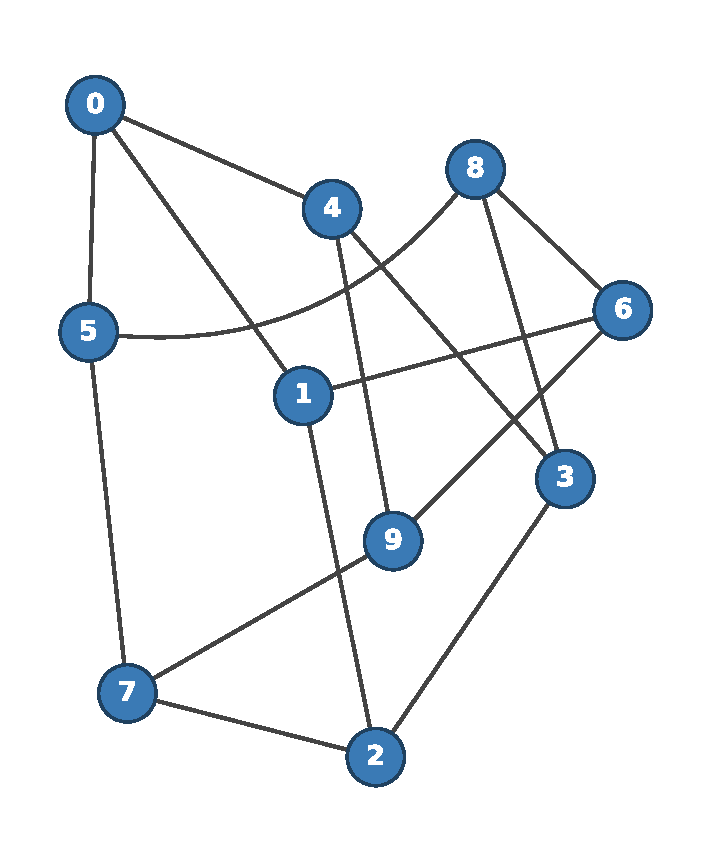
\includegraphics[width=0.52\textwidth]{fig_p1_q1_graph.pdf}
  \caption{Q1: the undirected graph on $10$ vertices and $15$ edges, drawn with
  the same vertex placement as the figure in the assignment. The edge $(5,8)$ is
  bowed so that it is visibly distinct from the vertex $4$ it passes behind.}
  \label{p1:fig:q1}
\end{figure}

The visualization is shown in Figure~\ref{p1:fig:q1}. It uses the same vertex
positions as the drawing in the assignment, so the two can be compared directly.

\subsection*{Q2: Graph Modification (15 pts)}

Starting from the graph $G$ of Q1 we remove, in order,

\begin{enumerate}
  \item \textbf{node $1$}, which also deletes its three incident edges
        $(0,1)$, $(1,2)$ and $(1,6)$;
  \item \textbf{edge $(0,4)$};
  \item \textbf{edge $(0,5)$}.
\end{enumerate}

Five edges are removed in total, leaving the graph $H$ on nine vertices with
ten edges:

\[
E(H)=\bigl\{(2,3),\,(2,7),\,(3,4),\,(3,8),\,(4,9),\,(5,7),\,(5,8),\,(6,8),\,(6,9),\,(7,9)\bigr\}.
\]

\begin{center}
\begin{tabular}{lcc}
\toprule
 & Before (Q1) & After (Q2) \\
\midrule
Nodes & $10$ & $9$ \\
Edges & $15$ & $10$ \\
Connected components & $1$ & $2$ \\
\bottomrule
\end{tabular}
\end{center}

\paragraph{Remaining components.} The three edges at node $0$ were exactly
$(0,1)$, $(0,4)$ and $(0,5)$, and all three are removed by the three operations
above. Node $0$ is therefore left isolated, and the resulting graph has
\textbf{two} connected components:

\begin{center}
\begin{tabular}{clc}
\toprule
Component & Vertices & Size \\
\midrule
$C_1$ & $\{0\}$ & $1$ \\
$C_2$ & $\{2,\,3,\,4,\,5,\,6,\,7,\,8,\,9\}$ & $8$ \\
\bottomrule
\end{tabular}
\end{center}

$C_2$ contains all ten remaining edges and is connected; $C_1$ is the isolated
vertex $0$. The remaining graph is drawn in Figure~\ref{p1:fig:q2}, using the
same vertex positions as Figure~\ref{p1:fig:q1} so that the effect of the
modification is directly visible; the isolated vertex $0$ is drawn in orange.

\begin{figure}[H]
  \centering
  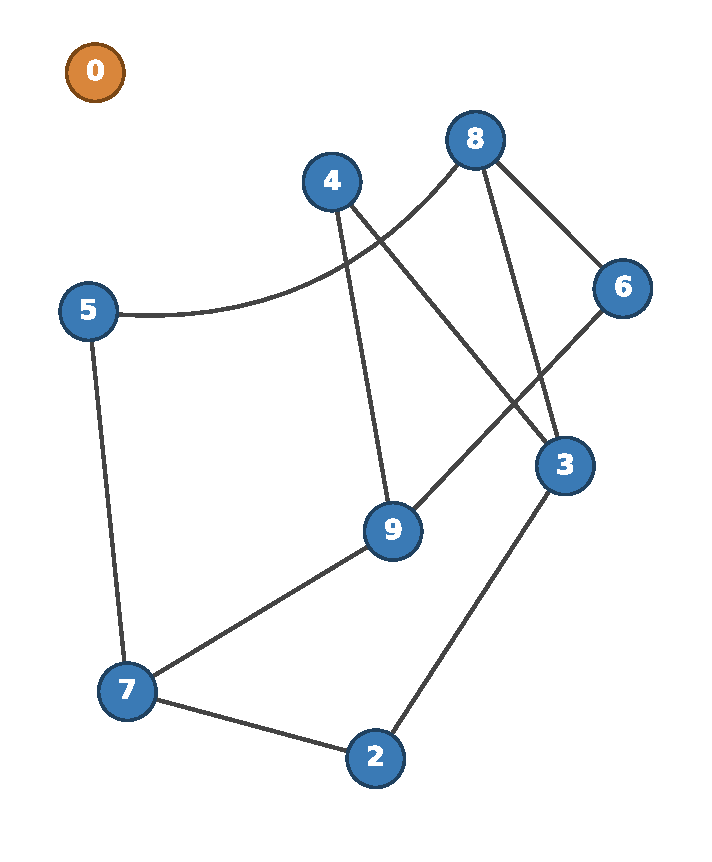
\includegraphics[width=0.52\textwidth]{fig_p1_q2_graph.pdf}
  \caption{Q2: the graph after removing node $1$ and the edges $(0,4)$ and
  $(0,5)$. Vertex positions are unchanged from Figure~\ref{p1:fig:q1}. The two
  connected components are the isolated vertex $0$ (orange) and the remaining
  eight vertices.}
  \label{p1:fig:q2}
\end{figure}
